\paragraph{Entrada al modelo y objetivos}

La entrada principal al modelo se puede resumir como en el esquema de la Figura \ref{fig:Esquema_preprocess_modelo}:

\begin{figure}[H]
    \centering
    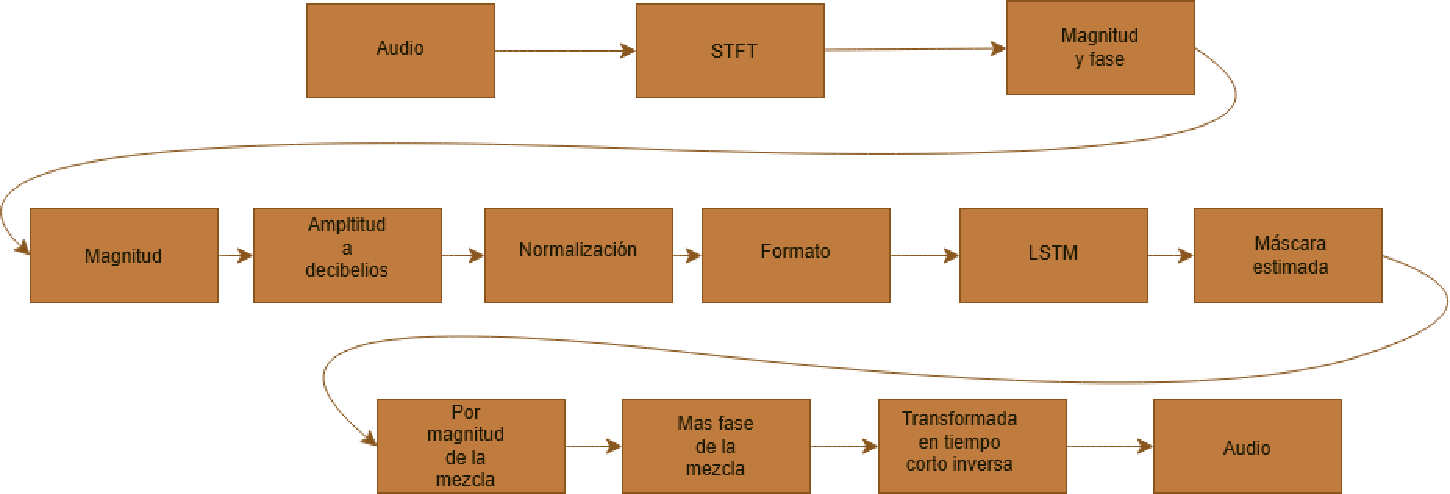
\includegraphics[
        width=\textwidth,
        keepaspectratio
    ]{commons/diagrama_procesado.drawio.pdf}

    \caption{Esquema del proceso de inserción de datos al modelo de inferencia de máscaras.}
    \label{fig:Esquema_preprocess_modelo}
\end{figure}

   
La estructura de entrada al modelo o \textit{input} es un vector que contiene:

\begin{itemize}
    \item \(B\): tamaño del \textit{batch}, es decir, número de ejemplos procesados simultáneamente.
    \item \(T\): número de frames temporales del espectrograma.
    \item \(F\): número de bins de frecuencia obtenidos mediante la STFT.
\end{itemize}

\begin{center}
    \[
[B, T, F]
\]
\end{center}

Y la estructura de salida o \textit{targets} es otro vector que contiene:

\begin{center}
  \[
[B, T, F, C, S]
\]  
\end{center}

Donde:

\begin{itemize}
    \item \(B\): tamaño del batch.
    \item \(T\): número de frames temporales.
    \item \(F\): número de bins de frecuencia.
    \item \(C\): número de canales de audio. En este trabajo es una constante \(C=1\), ya que las señales de entrada se transforman a mono por indicación de la documentación como ya se ha comentado en la sección anterior.
    \item \(S\): número de fuentes o \textit{stems} a separar. En este trabajo puede ser \(S=2\) para voz y acompañamiento, o \(S=4\) para voz, bajo, batería y resto.
\end{itemize}

La salida del modelo no genera audio directamente, la salida son máscaras tiempo-frecuencia. Posteriormente, se aplica la máscara sobre la magnitud de la mezcla y el resultado corresponde a una estimación de la magnitud de la fuente.
Luego para reconstruir el audio se utiliza la fase de la pista original. Esto es una limitación importante, ya que es una estimación. La fase de la mezcla original no tiene por qué ser la de las fuentes estimadas, pero a falta de este valor, se utiliza la fase de la mezcla como estimación de este último dato.

Los targets (objetivos) son las magnitudes de las fuentes reales, separados en los grupos de dos y cuatro fuentes que se han explicado en la sección anterior de este capítulo.





